\section{Introduction}
\label{sec:intro}






\begin{figure}[t]
  \centering
  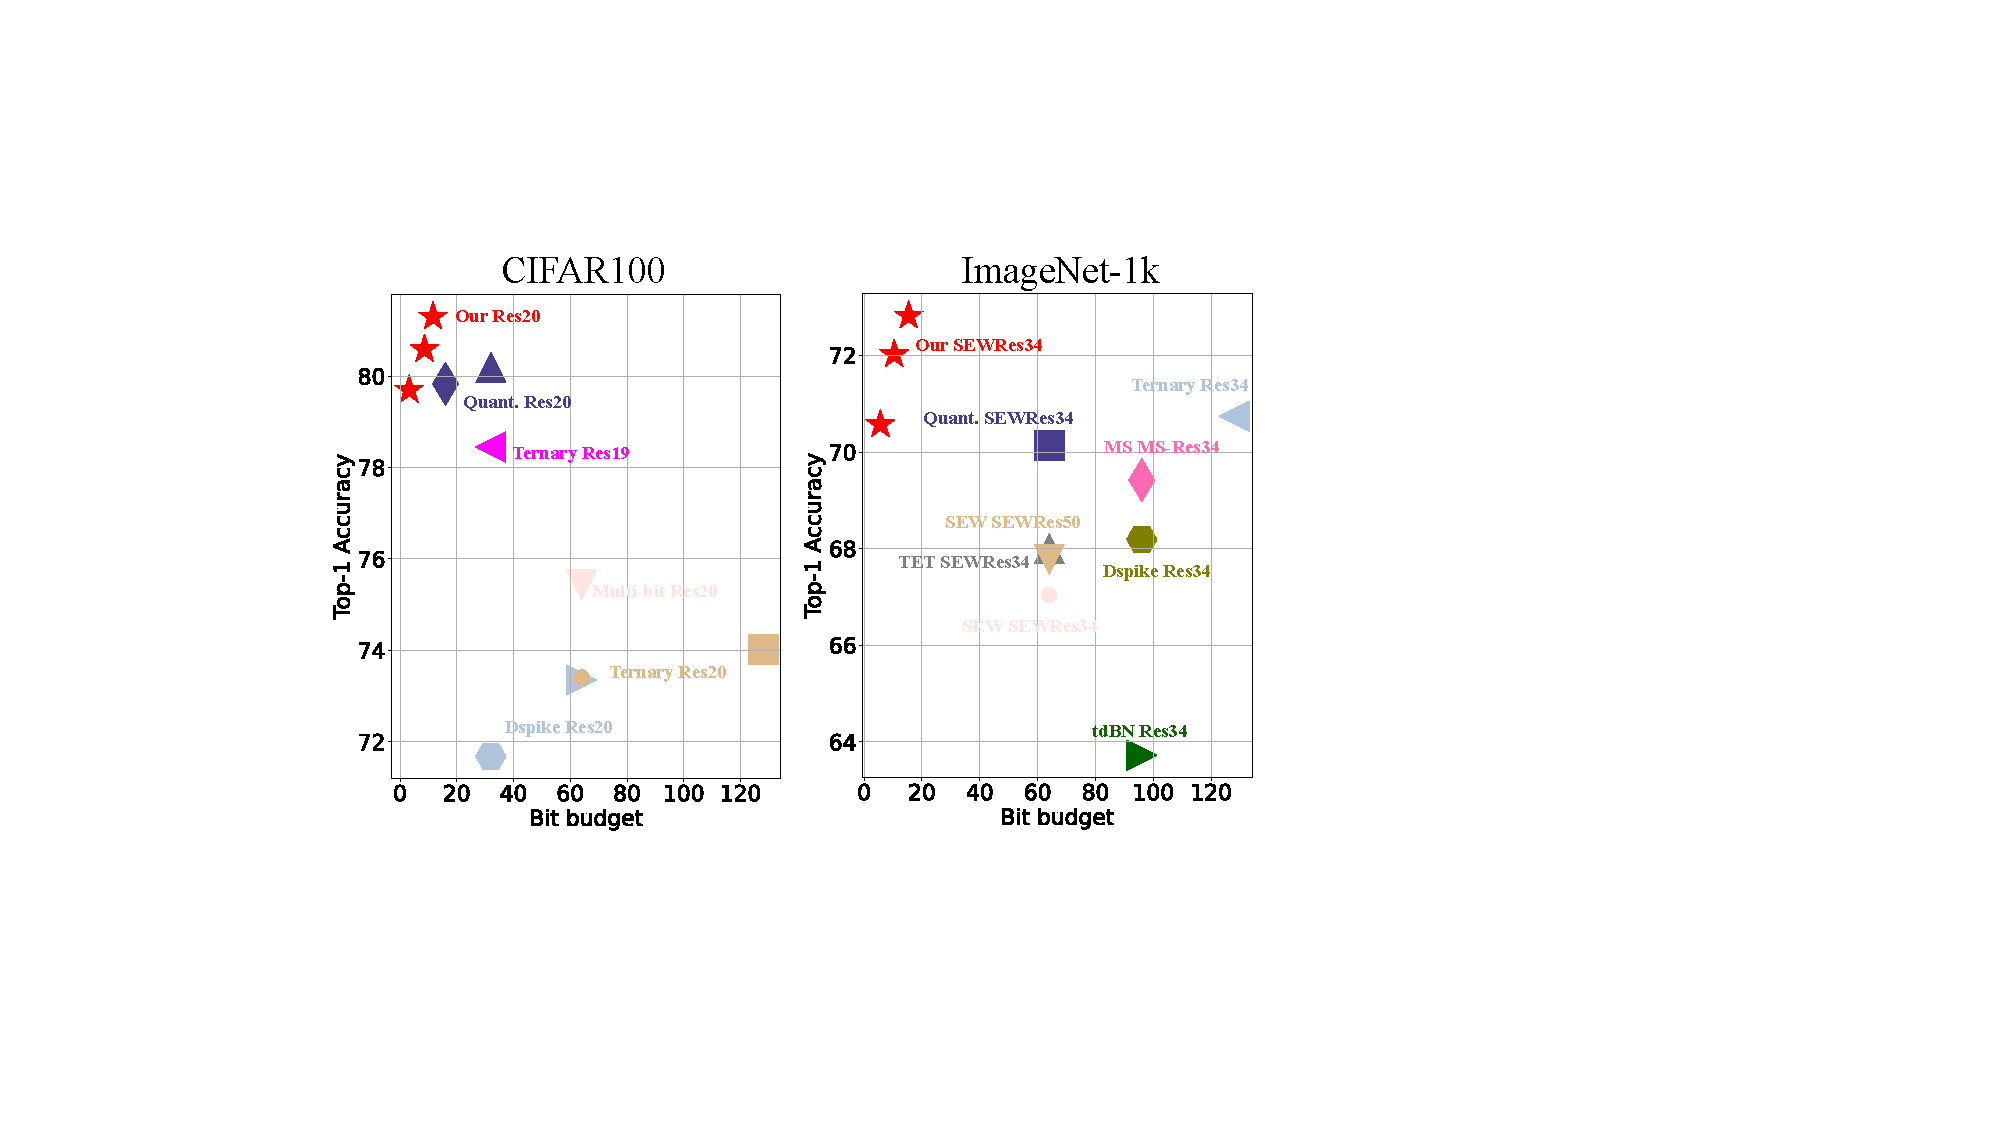
\includegraphics[width= 8cm]{figs/intro.pdf}
  \caption{Comparisons with other advanced SNNs using ResNet-based architectures on CIFAR100 and ImageNet-1k. Our models maintain the same level of model size as our baselines.}
  \label{fig:intro}
\end{figure}


Spiking neural networks (SNNs) are considered the third generation of neural networks \cite{maass1997networks}. The essential uniqueness of SNN is its activation unit, \ie, spiking neuron, that transfers the float value into binary spike, thus making the matrix operations, \eg, convolution, conducted in a multiplication-free way \cite{fang2021deep}. Similar to binary neural networks (BNN), binary feature maps (spikes) result in a reduction in spatial representation ability, making it challenging to process information-dense data and resulting in lower model accuracy \cite{zhu2019binary, meng2022training,zhou2022spikformer}.

Such being the case, multi-bit spiking neural networks have recently arisen as a promising approach to improving such inadequate informational scope \cite{guo2024ternary, xing2024spikellm,xing2024spikelm,xiao2024multi}. As the name suggests, multi-bit SNNs introduce more bits to represent the original binary spike and devote more addition operations to process the matrix multiplication. Prior arts successfully incorporate this mechanism to improve accuracy, while most of them neglect the actual memory and computation overhead as pointed out by  \cite{shen2024conventional}.
For example, a layer with less representation ability but assigned with high bit width would incur memory and computation waste and interfere the model inference \cite{dong2019hawq,Chen_2021_ICCV}. 
It desperately comes to the 
question: \emph{could we boost the performance of SNNs while maintain a constrained low-level memory and  computation overhead?} 

\begin{figure*}[t]
  \centering
  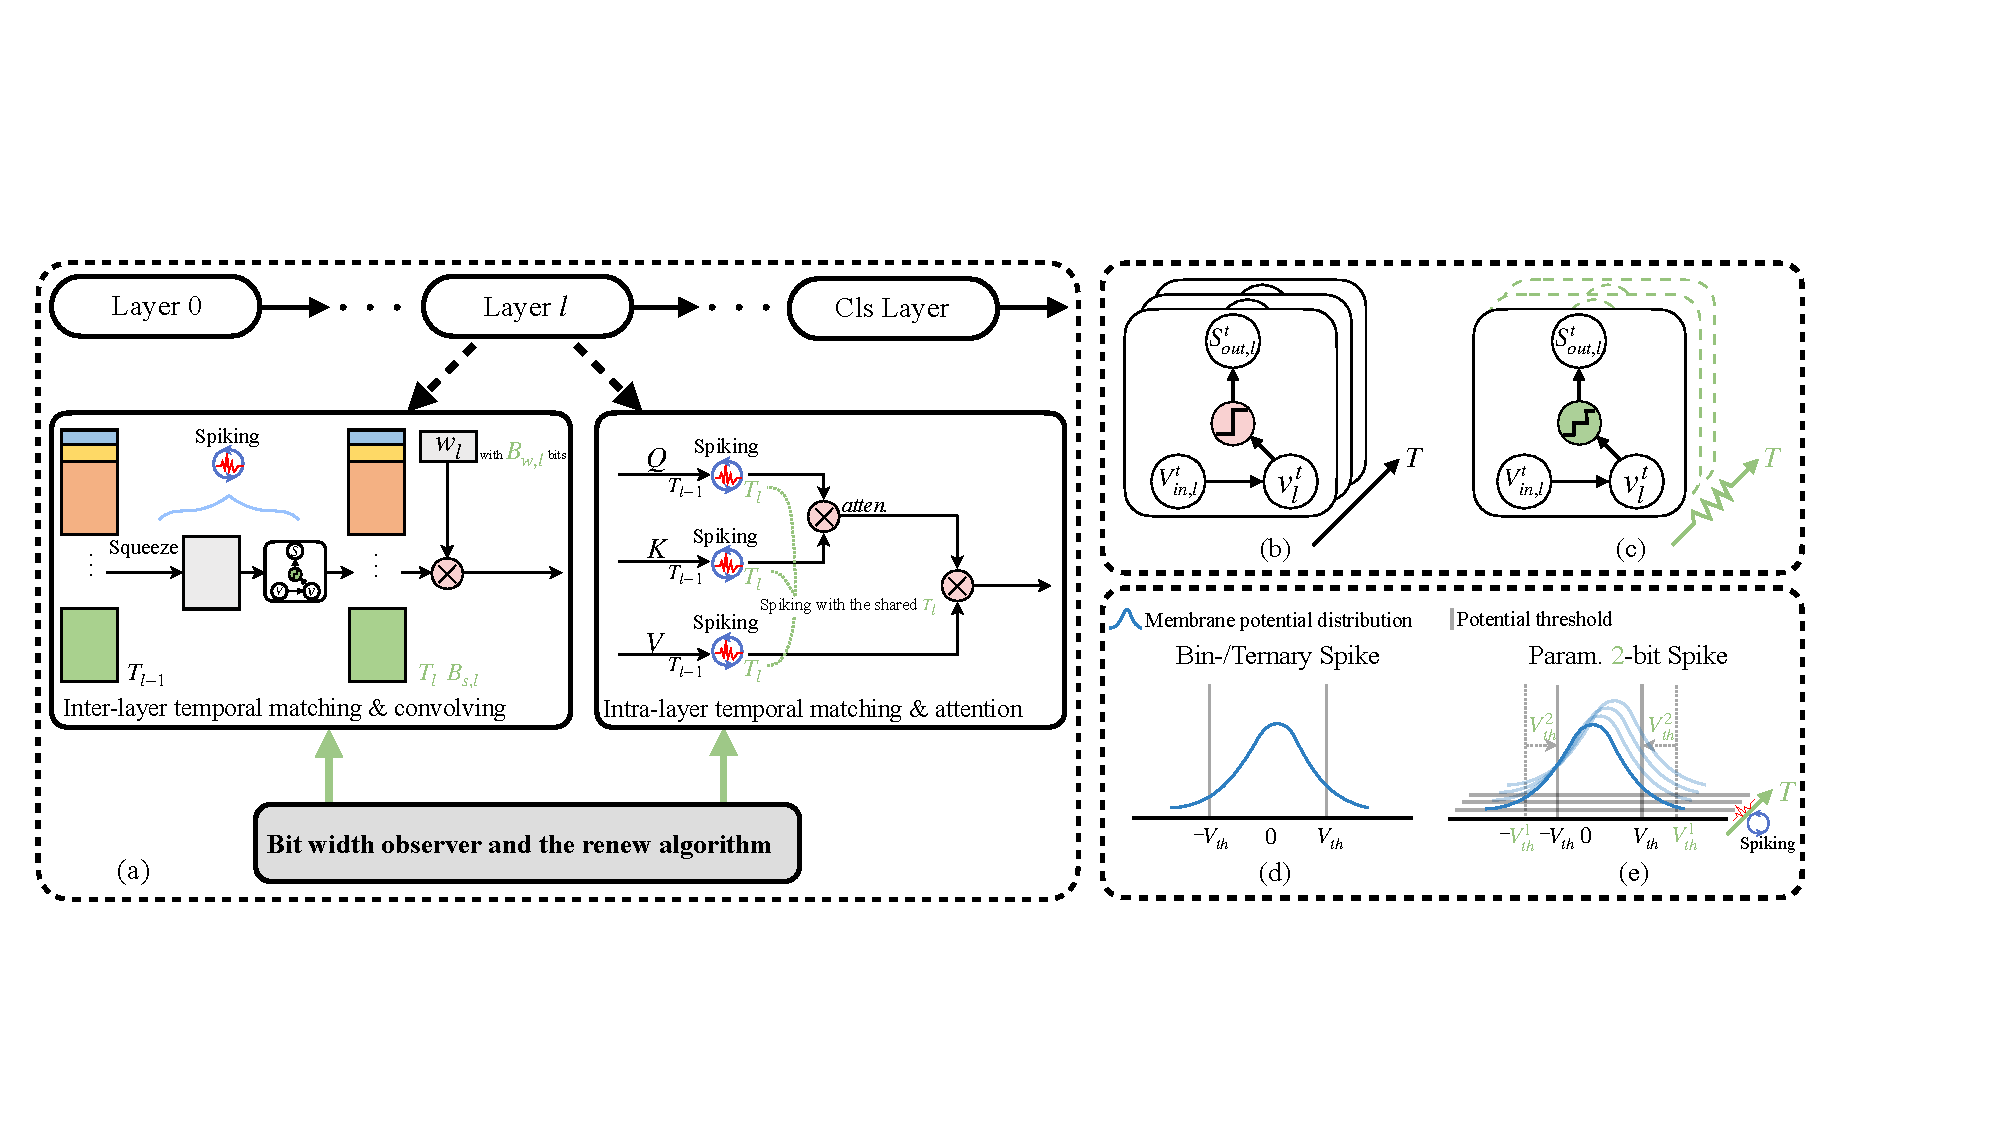
\includegraphics[width= 16cm]{figs/overview.pdf}
  \caption{Overview of the  proposed  bit allocation method. Green notations denote the parametrized constants. \textbf{(a)} Adaptive-bit-allocation training pipline, where the bit widths $T_l$, $B_{s,l}$, and $B_{w,l}$ are made learnable. $T_l$ is matched inter- and intra-layer to ensure the sufficient and fluent dataflow. The step-size renew mechanism is also proposed to alleviate the step-size mismatch issue. \textbf{(b)} and \textbf{(d)} depict the neuron formulation and the potential division of the previous binary and ternary spiking neuron, respectively. \textbf{(c)} and \textbf{(e)} depict our refined multi-bit spiking neuron, where the temporal length $T_l$ is layer-wise learnable and a shift $V^2_{th,l}$ is added to the potential threshold $V^1_{th,l}$. }
  \label{fig:overview}
\end{figure*}
In this paper, we investigate the adaptive bit allocation to answer this question. Specifically, we incorporate the pragmatic concept “Bit Budget” proposed by  \cite{shen2024conventional} and parametrize the three fundamental elements of bit budget: the bit widths of weights, spikes and temporal lengths, which also means the whole model is quantized. Thus, we can estimate the accurate model memory and computation by averaged bit width (Bit budget) and combined addition operation (S-ACE).
We then solve those non-differentiable terms to make these bit widths become learnable and can be optimized by the task loss signal. 
To constrain the changing of bit widths, we explicitly set bit bounds and implicitly design the bit width  loss to make the bit widths converge to the target widths correctly.

However, the special temporal dimension of SNN would pose new challenges. Firstly, the temporal dimension originally does not get involved in the forward pass, thus 
failing to get gradients for optimization. 
Secondly, previous multi-bit spiking neuron is designed and tuned chaotically, showing less friendliness to quantization. Thirdly, the potential step-size mismatch issue of learnable bit widths may become more severe as the temporal dimension
would consecutively use a wrong step size.
As illustrated in  \cref{fig:overview}, we first refine the spiking neuron, making it able to tackle temporal length mismatch inter- and intra-layer caused by changeable temporal length, and reducing quantization error via better formulations and potential divisions.
Then, we theoretically formulate the quantization step-size mismatch issue, where SNN would suffer a more severe offset that accumulates along the temporal dimension. Accordingly,
we propose the step-size renew mechanism, which consists of a bit-width observer and the renew algorithm. When the existence of the step-size mismatch is observed, the renew algorithm will be triggered to mend up step sizes automatically, ensuring a better training forward pass.


For the proposed theory and techniques, we conduct thorough experiments to prove the effectiveness. In comparisons with prior arts, we demonstrate that our method can achieve the SoTA performance with lower bit budgets as shown in  \cref{fig:intro}.

In summary, our contributions are as follows:

\begin{itemize}
    \item We propose an adaptive bit allocation method to build high-performace SNNs with low bit budgets. To the best of our knowledge, this is the first work that realizes an adaptive bit allocation for SNNs with direct training. 
    \item We accordingly refine the spiking neuron formulation to make full use of paramtrization and temporal information, and achieve better experimental results in the adaptive bit allocation.
    \item We theoretically formulate the step-size mismatch issue that could severely harm the training of SNNs, and
    propose the step-size renew mechanism to alleviate this issue, thus improving the overall model performance.
    \item We conduct thorough experimentation to demonstrate our proposed method's 
    effectiveness on both static and dynamic datasets. Comparative experiments also show that our model can achieve advanced accuracy with lower bit budgets as shown in \cref{fig:intro}. 
\end{itemize}


